\documentclass[11pt]{article}
\usepackage[utf8]{inputenc}
\usepackage{lingmacros}
\usepackage{tree-dvips}
\usepackage{enumitem}
\usepackage{graphicx}
\usepackage{titlesec}
\usepackage[bottom]{footmisc}
\graphicspath{ {./images/} }

\title{Rapport de stage Miguel Antoons}
\author{Miguel Antoons}

\begin{document}

\begin{titlepage}
    \begin{center}
        \LARGE
        \textbf{EPHEC}

        \vspace{0.1cm}
        \LARGE
        Technologie de l'Informatique

        \large
        \vspace{1.5cm}
        \textsc{Avenue du Ciseau 15}\\
        \textsc{1348 Ottignies-Louvain-la-Neuve}

        \vspace*{\stretch{1.0}}

        \line(1,0){350}\\
        \Huge
        \textbf{Rapport de Stage}\\
        \line(1,0){350}\\

        \vspace{0.5cm}
        \Large
        \textit{Miguel Antoons}

        \vspace{0.5cm}
        \large
        2021-2022

        \vspace{2.5cm}
        \large
        \textbf{Maitres de Stage}
        \vspace{0.2cm}\\
        Monsieur Hervé \textsc{Lamy}\\
        Monsieur Antoine \textsc{Calegaro}

        \vspace{2.5cm}
        \large
        \textbf{Professeur Rapporteur}
        \vspace{0.2cm}\\
        Monsieur Arnaud \textsc{Dewulf}


        \vspace*{\stretch{2.0}}
    \end{center}
\end{titlepage}

\tableofcontents

\newpage

\section{Remerciements}

Je tiens à remercier toutes les personnes qui m'ont aidé tout au long du stage et lors de la rédaction de ce rapport.\\
\\
En premier lieu, je remercie Mrs. Hervé Lamy et Antoine Calegaro. En tant que maîtres de stage, ils m'ont beaucoup appris et ont partagé leurs connaissances dans le domaine de l'informatique.\\
\\
Je remercie également mon professeur rapporteur, Mr. Arnaud Dewulf qui m'a permis de trouver ce stage et qui m'a suivi tout au long de son déroulement.\\
\\
Enfin, je voudrais exprimer ma reconnaissance envers toutes les personnes qui m'ont aidé lors de la rédaction et pour la relecture de ce rapport de stage.

\newpage

\section{Introduction}

\subsection{Objectifs du Stage}

Le stage d'insertion professionnelle proposé par l'Ephec a pour objectif de familiariser les étudiants avec le milieu dans lequel ils valoriseront leur diplôme.
Il permet de mettre en pratique la matière théorique vue tout au long du cursus en technologie de l'informatique grâce à la confrontation à des situations concrètes, mais également à l'aide de l'approche d'un professionnel.

\subsection{Attentes Personnelles}

Cette offre de stage a été proposée lors d'une présentation organisée par les membres du projet BRAMS, projet qui se déroule au sein de l'Institut Royal d'Aéronomie Spatiale de Belgique, durant le cours de traitement de signal donné par Mr Dewulf.
Ayant déjà contacté des sociétés, mais n'ayant pas encore pris de décision, j'ai décidé de prendre rendez-vous avec l'institut.\\
\\
Le travail principal proposé par l'institut était la migration d'un site web vers un autre framework.
L'ancien framework ainsi que le nouveau m'étant inconnus, ceci m'a attiré pour les nombreuses compétences à apprendre.\\
Ce stage, comme la plupart des stages, permettait également de voir comment un environnement professionnel s'organise et fonctionne.\\
\\
Enfin, n'étant plus dans un milieu scolaire, j'étais curieux quant à la complexité d'écrire des programmes complets, de qualité dans les délais imposés.
Ceci s'étend d'un débogage et une maintenance facilités pour le développeur qui viendra après moi, jusqu'au développement d'une interface conviviale et facile à utiliser pour l'utilisateur.
Cette attente était d'autant plus intéressante sachant que j'allais devoir apprendre un nouveau langage et un nouveau framework durant ces délais.

\newpage

\section{Institut Royal d'Aéronomie Spatiale de Belgique}

L'institut Royal d'Aéronomie Spatiale de Belgique ou IASB est un institut scientifique fédéral belge fondé le 25 novembre 1964.
Il est situé sur le plateau d'Uccle, où se situent également d'autres instituts scientifiques, à savoir l'Institut Royal Météorologique ou IRM et l'Observatoire Royal de Belgique.\\
\\
Les tâches principales de l'IASB sont, comme son nom l'indique, la recherche et les services publics dans le domaine de l'aéronomie spatiale.
L'aéronomie a pour objet l'étude des régions atmosphériques où les phénomènes de dissociations moléculaires et d'ionisation sont importants.
Par extension, l'aéronomie couvre aussi l'étude des comètes et d'autres planètes.
Leur objectif est d'élargir la connaissance des atmosphères des corps célestes.\\
\\
Parmi les activités de l'IASB, on retrouve le contrôle des expériences belges à bord de la station spatiale internationale et d'autres satellites, ou encore la conception d'instruments qui serviront à surveiller les atmosphères et l'environnement spatial.\\
\\
Quelques domaines de recherche de l'IASB :
\begin{itemize}[noitemsep]
    \item Le développement des missions spatiales,
    \item La qualité de l'air,
    \item La physique spatiale.
\end{itemize}
\vspace{10pt}
L'IASB est subdivisé en quatre départements, comme nous le montre la figure 1 :
\begin{itemize}[noitemsep]
    \item le département de physique spatiale,
    \item le département de composition atmosphérique (sources et pertes),
    \item le département de composition atmosphérique (gaz réactifs),
    \item le département de radiations solaires dans les atmosphères.
\end{itemize}
\vspace{3pt}

\begin{figure}[t]
    \begin{center}
        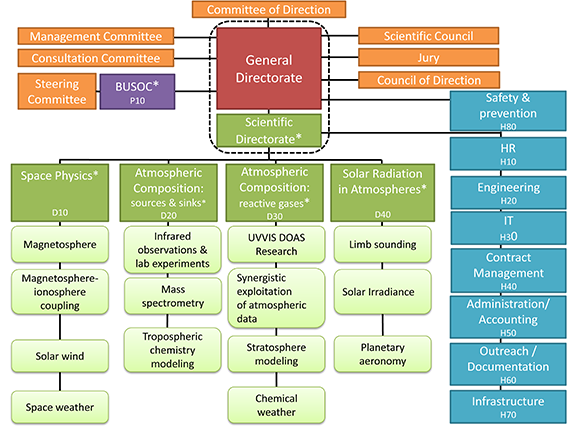
\includegraphics[scale=0.5]{organization.png}
        \caption{Organisation des départements de l'IASB}
    \end{center}
\end{figure}

\newpage

\subsection{Le projet BRAMS}

Le projet BRAMS (Belgian RAdio Meteor Stations) collecte et stocke des données relatives à des objets entrants dans l'atmosphère belge (météores entre autres).
Ces données sont ensuite analysées afin de pouvoir étudier plus précisément les trajectoires, la vitesse et éventuellement les masses des météores.\\
\\
Le projet a débuté en 2010 par Hervé Lamy à l'IASB, dans le département de physique spatiale.
Il dispose d'un réseau de stations émettrices et réceptrices radio nommé le réseau BRAMS.
Ce réseau fonctionne de la façon suivante :
\begin{enumerate}
    \item Un émetteur, situé à Dourbes, transmet de façon continue un signal à une fréquence fixe.
          Ce signal est émis en direction du ciel et peut être réfléchi sur des trainées ionisées dans le sillage des météores.
    \item Une fois réfléchi, le signal est, dans le cas idéal, détecté par une ou plusieurs récepteurs du réseau BRAMS.
          Chaque station de réception enregistre continuellement les données dans des fichiers son de type WAV\footnote{Waveform Audio File}.
          Toutes ces stations sont hébergées soit par des radio-amateurs qui veulent contribuer au projet, soit par des observatoires publics ou encore par l'IASB même.
    \item Les fichiers WAV sont envoyés à intervalles réguliers à l'institut via, dans la plus grande partie des cas, internet, ou parfois, via clé USB.
    \item Ces données sont ensuite archivées et étudiées par les personnes travaillant sur le projet.
          Afin de pouvoir mieux visualiser les données, on génère des spectrogrammes à partir des fichiers WAV.
          Un exemple de spectrogramme peut être visualisé sur la figure 2.
\end{enumerate}

\begin{figure}[t]
    \begin{center}
        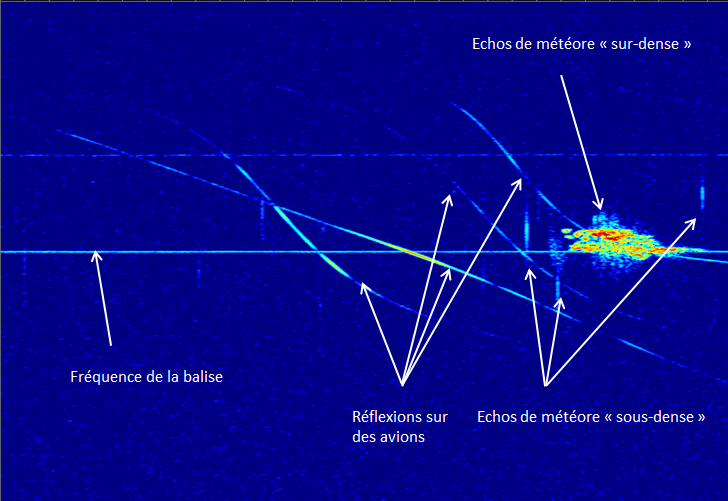
\includegraphics[scale=0.493]{spectrogramme.png}
        \caption{Exemple d'un spectrogramme venant des stations de réception}
    \end{center}
\end{figure}

\vspace{10pt}
Plus d'informations à propos du projet BRAMS sont disponibles en ligne, sur le site web du projet.\footnote{Accessible à l’adresse suivante : http://brams.aeronomie.be}

\newpage

\section{Nature du Stage}

Dans cette section, j'explique dans quel domaine de l'informatique j'ai principalement travaillé pendant le stage, ainsi que mes réalisations pour l'entreprise.\\
\\
Mon stage a démarré le 14 février et a pris fin le 20 mai. Durant toute cette période, j'ai travaillé sur le projet BRAMS.\\
\\
Ma tâche principale était l'amélioration et la migration vers un nouveau framework du site web du projet BRAMS.
L'ancien framework du site était CakePHP, le nouveau framework est Joomla. Tous deux framework utilisent le PHP comme langage back-end combiné avec du JavaScript, du HTML\footnote{HyperText Markup Language : permet de structurer les éléments sur le site} et du CSS\footnote{Cascading Style Sheets : permet de changer le style du site} pour fournir des fonctionnalités du côté front-end.\\
Le PHP étant un langage que je n'avais encore jamais utilisé, ceci impliquait l'apprentissage de ce langage avant de pouvoir m'attaquer au développement du site web.
La migration était nécessaire afin de permettre l'uniformité d'un seul et même framework au sein de tous les sites web de l'IASB.
Afin de compléter certaines fonctionnalités spécifiques du côté du front-end, il a également fallu utiliser de librairies open-source JavaScript.\\
\\
Plusieurs fois par semaine, je montrais mon avancement sur le site afin d'avoir un retour.
Ceci m'a permis de vraiment bien améliorer le site aux besoins des membres du projet BRAMS.
Durant les dernières semaines de stage, le site est passé dans une phase de test pour les utilisateurs.
Lors de cette période, les utilisateurs me faisaient part de leurs remarques sur le site, ou encore de certains points qui restent à améliorer.
Ceci a conduit à un site de qualité, facile à utiliser à la fois pour les membres du projet BRAMS ainsi que pour des personnes visitant le site à l'occasion.

\subsection{Réalisations}

Dans cette section, je passe en revue mes réalisations durant le stage.

\subsubsection{Pages statiques}
Joomla étant un CMS\footnote{Content Management System : outil permettant de créer des pages web à l'aide d'une interface graphique}, la réécriture des pages statiques de l'ancien site web s'est déroulée très rapidement.
Grâce à l'interface graphique, il suffisait de copier le texte brut de l'ancien site web, le mettre en forme et finalement, ajouter les images.
Joomla étant un framework qui propose des modèles avec une structure et un style déjà tout fait (HTML \& CSS), peu de travail me restait à faire sur ces 2 aspects.

\subsubsection{Visualisation de la disponibilité des données}

Étant donné la grande quantité de données qui est enregistrée quotidiennement, lorsqu'on désire accéder une donnée spécifique, un outil permettant de visualiser la disponibilité des données peut représenter un gain de temps non négligeable.
En effet, il y a à présent 42 récepteurs actives qui envoient chacun 288 fichiers (1 fichier tout les 5 min) par jour.
Il y a à présent plus de 30 millions de fichiers pour le projet BRAMS.
C'est pourquoi sur le site, un outil permettant la visualisation facile de la disponibilité des données pour chaque station existe.\\
\\
Cet outil a été créé à l'aide de la librairie JavaScript open source Visavail.js\footnote{https://github.com/flrs/visavail} et affiche la disponibilité des fichiers sous forme de code couleur.
Une des améliorations apportées à cet outil par rapport à l'ancien est la minimisation des données qui circulent sur le réseau.
En effet, la quantité des données demandée peut devenir très grande quand on veut visualiser la disponibilité sur une très longue période, ce qui cause un temps de chargement de plusieurs minutes.
Grâce à cette optimisation, ce temps de chargement ce réduit de plusieurs minutes à quelques secondes.\\
\\
Une autre amélioration apportée, et ceci pour tous les outils, et la diminution des rechargements de la page.
Tandis que l'ancien site rechargeait la page à chaque fois qu'un utilisateur voulait accéder à des données back-end, le nouveau site fonctionne avec des API\footnote{Application Program Interface : connexion entre différents programmes informatiques} et cherche uniquement les données nécessaires au lieu de recharger toute la page.
C'est non-seulement une expérience plus agréable pour l'utilisateur, mais permet aussi d'économiser de la bande passante réseau.\\
\\
L'outil de visualisation de la disponibilité des données était le premier outil dynamique que j'ai dû développer pour le site web.
Ceci s'est ressenti dans le temps que j'ai mis afin d'arriver à une version définitive de la nouvelle version.
En effet, durant le développement de cet outil, j'ai non-seulement dû me familiariser avec PHP et l'organisation MVC\footnote{Model-View Controller : Façon d'organiser le code en séparant la partie donnée, la partie interface et la partie logique.} de Joomla mais également avec les systèmes informatiques de l'institut.\\
\\
Un exemple de l'outil de visualisation de la disponibilité des données BRAMS est affiché sur la figure 3.

\begin{figure}[t]
    \begin{center}
        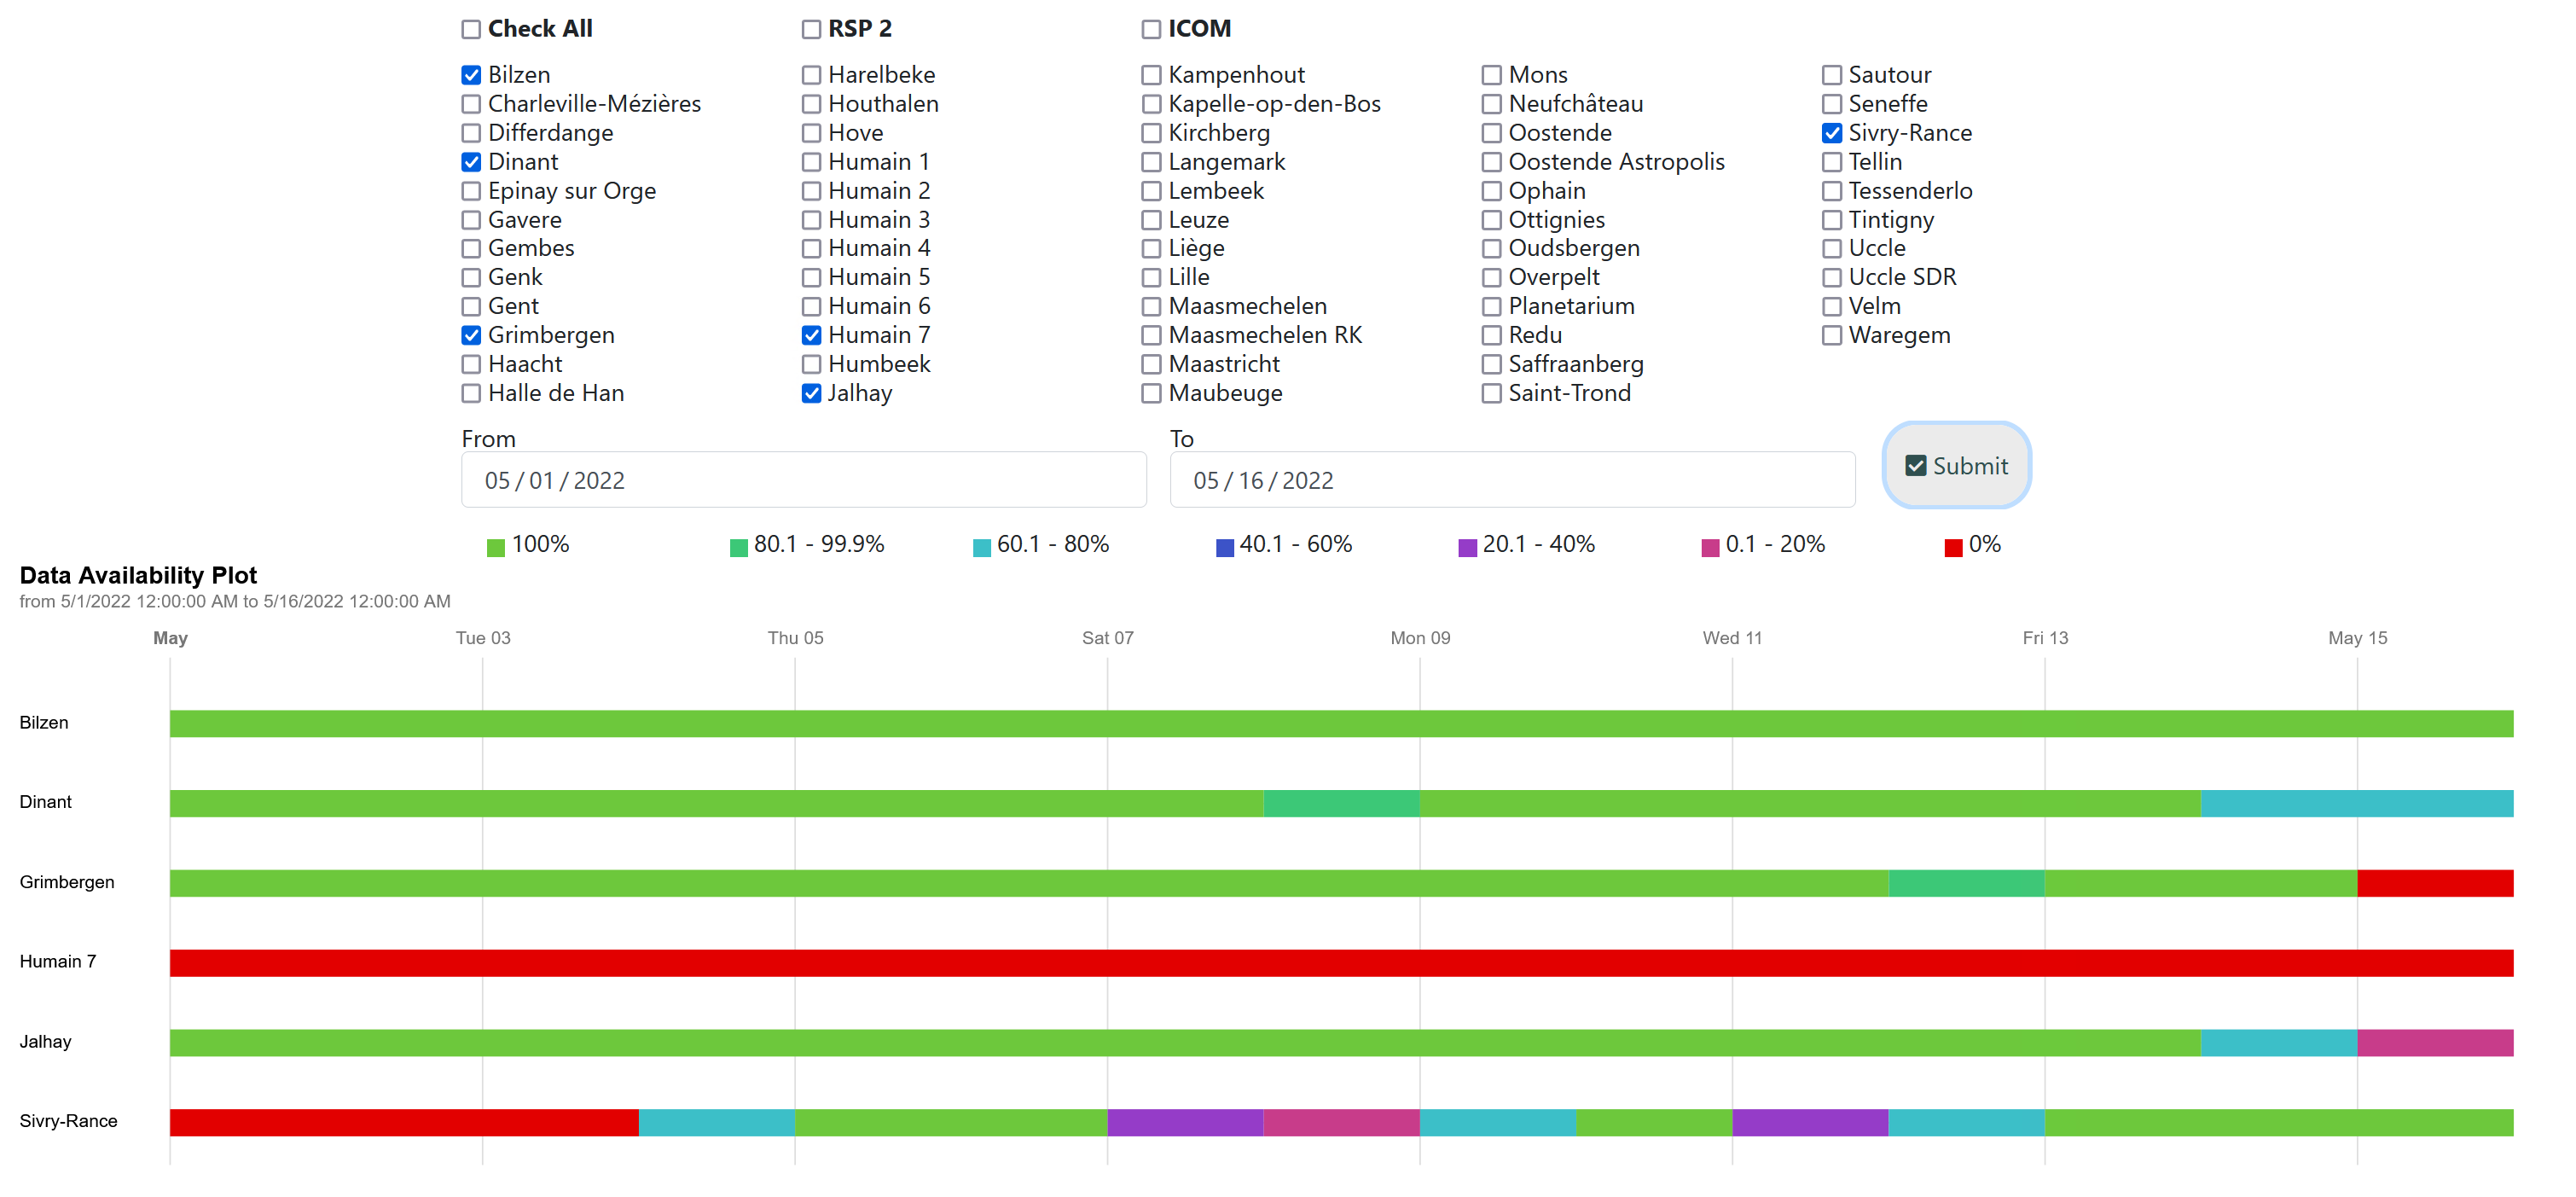
\includegraphics[scale=0.155]{availability.png}
        \caption{Outil de visualisation de la disponibilité des fichiers pour chaque station}
    \end{center}
\end{figure}

\subsubsection{Data Viewer}

Dans le but de permettre aux utilisateurs, autant internes qu'externes au projet BRAMS, de visualiser les données générées par les stations, un outil qui porte le nom de Data Viewer a été mis en place.
Cet outil permet d'afficher les spectrogrammes de différentes stations dans un intervalle défini par l'utilisateur ainsi que le téléchargement du spectrogramme et du fichier WAV auquel le spectrogramme est associé.
Ceci permet de comparer les données plus facilement entre les différentes stations.\\
\\
Le Data Viewer utilise la librairie open source Viewer.js\footnote{https://fengyuanchen.github.io/viewerjs/} qui permet d'afficher les images en grand ainsi que la navigation entre les images.
La plus grande amélioration apportée à ce programme est au niveau de l'interface.
Pour des utilisateurs n'ayant pas la connaissance de comment utiliser le programme, la sélection de période ainsi que des différentes stations pouvait être difficile.
Moi-même, la première fois que j'ai voulu utiliser le programme j'ai dû demander de l'aide puisque je pensais qu'il ne fonctionnait pas.
Ce problème est résolu et le programme est maintenant plus facile à utiliser par rapport à la version précédente.\\
\\
Un exemple du BRAMS Data Viewer se trouve sur la figure 4.

\begin{figure}[t]
    \begin{center}
        \includegraphics[scale=0.154]{viewer.png}
        \caption{BRAMS Data Viewer}
    \end{center}
\end{figure}

\subsubsection{Carte dynamique des stations}

Afin de pouvoir visualiser l'évolution et l'état du réseau BRAMS, le site web dispose d'une carte dynamique de la Belgique.
Une des améliorations apportées à cette page est la possibilité de voir le réseau BRAMS à une date précise.
La nouvelle version permet également de représenter un type de station précis et représente aussi le pourcentage de données disponible pour le jour sélectionné.
Chaque station est représentée par un point vert s'il dispose de données pour ce jour-là ou un point rouge dans le cas contraire.\\
\\
Afin de pouvoir afficher des points à des endroits précis sur une image, la librairie open source maphighlight\footnote{https://github.com/kemayo/maphilight} a été utilisé.
Une capture d'écran de l'outil peut être visualisé sur la figure 5.

\begin{figure}[t]
    \begin{center}
        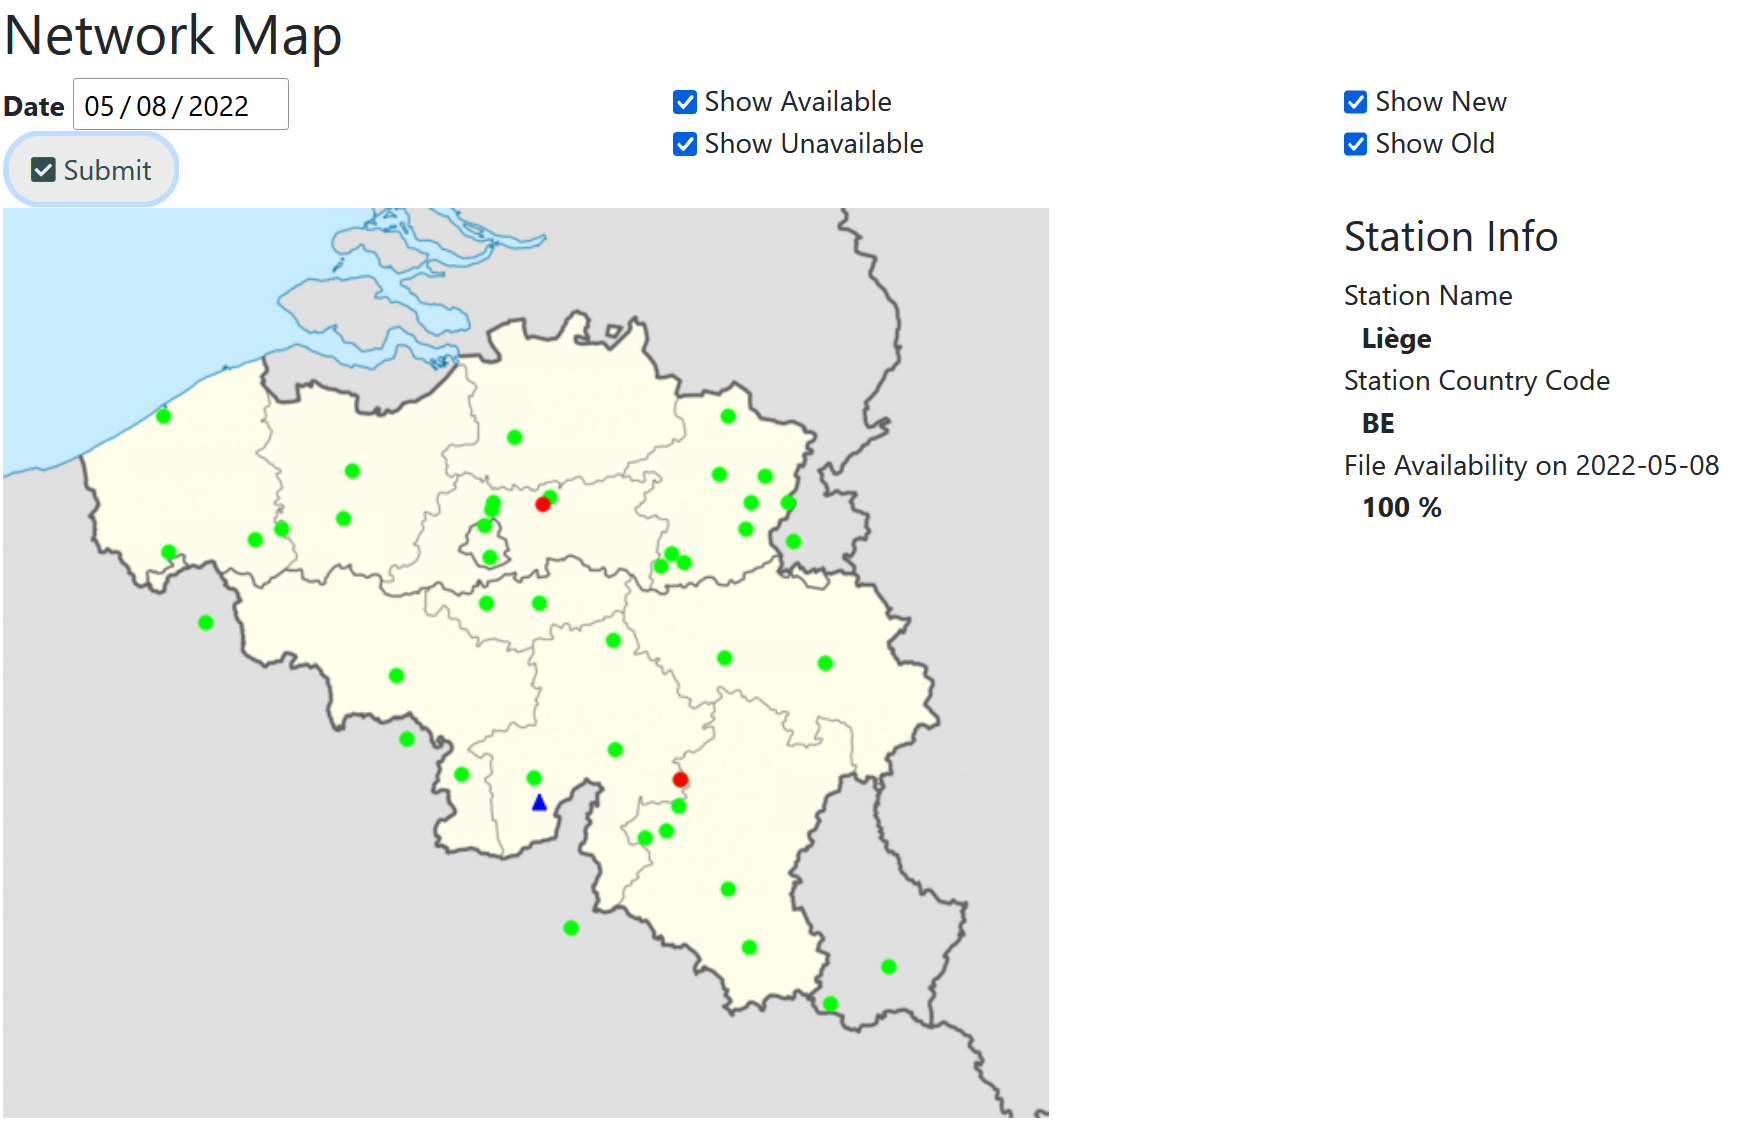
\includegraphics[scale=0.25]{map.png}
        \caption{Carte dynamique du réseau BRAMS}
    \end{center}
\end{figure}

\subsubsection{Campagnes BRAMS}

Dans le but de mettre en évidence les météores sur les spectrogrammes, un outil nommé BRAMS Campaigns avait été développé sur l'ancien site web du projet BRAMS.
Cet outil donnait la possibilité aux membres du projet BRAMS de tracer des carrés autour des météores et de télécharger les spectrogrammes ensemble avec les carrés.
Cependant, cet outil ne fonctionnait plus depuis quelque temps.\\
\\
C'est alors lors du développement de la nouvelle version du programme que je me suis aperçu du même problème or le code était complètement différent.
Après une recherche pour trouver la cause du problème, je me suis aperçu qu'une des tables impliquée dans l'outil disposait d'un moteur de base de données différent des autres.
Les autres tables utilisant tout le moteur InnoDB de MySQL, cette table particulière utilisait le moteur plus ancien MyISAM, également de MySQL.\\
\\
Ce changement avait été fait il y a quelque temps avant mon stage afin de développer un nouvel outil pour le projet BRAMS.
Le problème était que MyISAM ne supportait pas les clés étrangères, or lors du changement du moteur vers MyISAM, les clés étrangères existantes sur la table n'ont pas été suprimmés.
Ceci empêchait la création d'une nouvelle campagne et rendait le programme inutilisable.\\
\\
J'ai développé le côté front-end du site en me basant sur le code déjà existant.
Cependant, j'ai apporté des améliorations aux enregistrements des carrés tracés, qui se fait maintenant de façon continue au lieu de devoir appuyer sur un bouton pour enregistrer tous les carrés tracés sur un spectrogramme.

\subsubsection{Outils d'Administration}

Le développement de plusieurs pages permettant l'ajout, la modification et la suppression de données dans la base de données fut également nécessaire.
Pour chaque table nécessitant des modifications des données par le site, deux pages étaient développées.
Une page contenant un tableau avec toutes les données dans cette table et un bouton pour ajouter une rangée qui redirige l'utilisateur vers un formulaire d'ajout.
Chaque rangé dans la table sur la page représente une rangée dans la base de données et contient un bouton 'modifier' et un bouton 'supprimer'.\\
\\
Quand l'utilisateur clique sur le bouton 'modifier' il est redirigé vers le même formulaire que celui pour ajouter une rangée, mais cette fois le formulaire est préremplis avec les données de la rangée dans la base de données que l'on souhaite modifier.
Les améliorations apportées à ces pages portent surtout sur un nouveau design plus simple et moderne ainsi que l'automatisation ou encore l'ajout des valeurs par défaut pour les champs des formulaires.\\
\\
Les changements d'une page d'administration à un autre étant minimales, ceci a causé beaucoup de tâches répétées.
En effet, il y avait huit tables pouvant être manipulés depuis le site chacun nécessite deux pages.
Ceci rendait le développement de ces pages beaucoup moins intéressant.

\newpage

\section{Expériences Vécues}

Avec les mesures prises suite au COVID, faire connaissance avec mes collègues s'est avéré plus compliqué au début.
Néanmoins, dès mon arrivée j'y ai été accueilli agréablement ce qui m'a permis de rapidement m'intégrer dans l'équipe.\\
\\
On m'a attribué un bureau à moi avec un espace suffisant et une vue vers l'extérieur très agréable.
Ceci avait l'avantage qu'étant seul, je pouvais me concentrer à 100 \% sur mon travail sans être dérangé.
D'un autre côté, avec les mesures du COVID, je passais parfois des journées seul sans voir mes collègues.
Heureusement, ça s'est amélioré avec les semaines qui passaient et l'assouplissement des mesures contre le COVID.\\
\\
Lors de mon stage, j'ai également été en contact avec des employés d'autres départements au sein de l'IASB afin de m'aider dans mes tâches.
Lorsque j'avais une question, je savais m'adresser à mes collègues du projet BRAMS, ou encore, aller voir les membres du département informatique.
Ceci m'a aidé notamment au début de mon stage, quand j'ai rencontré un problème empêchant Joomla de fonctionner correctement.
Joomla n'avait aucun droit d'écriture, ce qui bloquait toute installation de pages dynamique ou encore de modèles graphiques.
C'était également l'occasion d'apprendre à se connaître en discutant de sujets divers.\\
\\
Plusieurs fois par semaine Mr Antoine Calegaro, mon maître de stage, venait voir mon avancement sur le site.
Ceci m'a permis de m'améliorer dans mon travail et d'apprendre des nouvelles choses auxquelles je n'avais pas encore fait attention.\\
\\
Enfin, l'institut étant situé à un endroit très vert et calme, l'environnement de travail y était vraiment agréable.

\newpage

\section{Conclusion}

Durant la période de stage, j'ai eu l'occasion d'apprendre de nombreuses choses, mais avant tout j'ai pu me former une idée plus précise de quel type de travail me conviendrait.\\
\\
J'ai pu finaliser le travail demandé, mais j'ai mis plus de temps que prévu causant le site à être en phase de test lorsque je dépars de mon stage.
Ceci est en partie causé par les problèmes avec l'infrastructure de l'institut m'empêchant de développer de façon efficace le site durant les premières semaines, mais également par mon manque d'organisation durant les premières semaines.
Ces deux problèmes ont heureusement évolués de façon positive afin d'arriver à un bon résultat.\\
\\
Je suis satisfait de mon travail et de mon évolution durant cette période et également du fait que le travail réalisé sera utile à grand nombre de personnes.
Je sors du stage avec des nouvelles compétences techniques acquises, des nouvelles personnes rencontrées, une meilleure connaissance de moi-même et une meilleure aptitude à m'organiser pour finir un travail dans des délais imposés.\\
\\
Ce stage clôture donc parfaitement mes études à l'EPHEC et permettra de mieux m'orienter dans les années à venir.

\end{document}
